\documentclass{beamer}
\usepackage[utf8]{inputenc}

\usetheme{Madrid}
\usecolortheme{default}
\usepackage{amsmath,amssymb,amsfonts,amsthm}
\usepackage{txfonts}
\usepackage{tkz-euclide}
\usepackage{listings}
\usepackage{adjustbox}
\usepackage{array}
\usepackage{tabularx}
\usepackage{gvv}
\usepackage{lmodern}
\usepackage{circuitikz}
\usepackage{tikz}
\usepackage[utf8]{inputenc}

\usetheme{Madrid}
\usecolortheme{default}
\usepackage{amsmath,amssymb,amsfonts,amsthm}
\usepackage{txfonts}
\usepackage{tkz-euclide}
\usepackage{listings}
\usepackage{adjustbox}
\usepackage{array}
\usepackage{tabularx}
\usepackage{gvv}
\usepackage{lmodern}
\usepackage{circuitikz}
\usepackage{tikz}
\usepackage{graphicx}

\setbeamertemplate{page number in head/foot}[totalframenumber]

\usepackage{tcolorbox}
\tcbuselibrary{minted,breakable,xparse,skins}



\definecolor{bg}{gray}{0.95}
\DeclareTCBListing{mintedbox}{O{}m!O{}}{%
  breakable=true,
  listing engine=minted,
  listing only,
  minted language=#2,
  minted style=default,
  minted options={%
    linenos,
    gobble=0,
    breaklines=true,
    breakafter=,,
    fontsize=\small,
    numbersep=8pt,
    #1},
  boxsep=0pt,
  left skip=0pt,
  right skip=0pt,
  left=25pt,
  right=0pt,
  top=3pt,
  bottom=3pt,
  arc=5pt,
  leftrule=0pt,
  rightrule=0pt,
  bottomrule=2pt,

  colback=bg,
  colframe=orange!70,
  enhanced,
  overlay={%
    \begin{tcbclipinterior}
    \fill[orange!20!white] (frame.south west) rectangle ([xshift=20pt]frame.north west);
    \end{tcbclipinterior}},
  #3,
}
\lstset{
    language=C,
    basicstyle=\ttfamily\small,
    keywordstyle=\color{blue},
    stringstyle=\color{orange},
    commentstyle=\color{green!60!black},
    numbers=left,
    numberstyle=\tiny\color{gray},
    breaklines=true,
    showstringspaces=false,
}
%------------------------------------------------------------
%This block of code defines the information to appear in the
%Title page
\title %optional
{1.9.3}
\date{August  2025}
%\subtitle{A short story}

\author % (optional)
{Bhoomika L - EE25BTECH11014}

\begin{document}


\frame{\titlepage}
\begin{frame}{Question}\textit{AOBC} is a rectangle whose three vertices are $\brak{0,-3}$ $\brak{0,0}$ $\brak{4,0}$.The length of its diagonal is\rule{2cm}{0.4pt}
\end{frame}

\begin{frame}{Theoretical Solution}

 Given the points $\vec{A},\vec{O}$ and $\vec{B}:$\\
\begin{table}[H]    
  \centering
  \begin{tabular}{|c|c|c|c|}
\hline
Angle (\(\alpha\)) & \(\cos(\alpha)\) & Value & Axis \\
\hline
\(90^\circ\) & \(\cos(90^\circ) = 0\) & \(l = 0\) & x-axis \\
\(60^\circ\) & \(\cos(60^\circ) = \frac{1}{2}\) & \(m = \frac{1}{2}\) & y-axis \\
\(30^\circ\) & \(\cos(30^\circ) = \frac{\sqrt{3}}{2}\) & \(n = \frac{\sqrt{3}}{2}\) & z-axis \\
\hline
\end{tabular}
  \caption{Position Vectors of the points on rectangle.}
  \label{tab:1.9.3}
\end{table}

\end{frame}


\begin{frame}{Theoretical Solution}
Determining the Coordinates of Point C:
\begin{align}
 \vec{A} = \myvec {4\\0 }
 \vec{B} = \myvec {0\\-3}
\end{align}
 Since $\vec{C}$ is opposite to $\vec{O}$ in the rectangle,
\end{frame}

\begin{frame}{Formulae}
\begin{align}
\vec{C} = \vec{A} + \vec{B}
\\
\implies \myvec{4\\0}+ \myvec{0\\-3}=\myvec{4\\-3}\\
\therefore \vec{C}=\myvec{4\\-3}
\end{align}
\end{frame}

\begin{frame}{Theoretical solution}

We know that the length of the diagonal vector is magnitude of the vector $\vec{C}$.\\

\begin{align}
\vec{C}= \myvec{4 \\ -3} 
\end{align}


\begin{align}
\left|\vec{C} \right| &= \sqrt{ \vec{C}^T \cdot \vec{C}}
 \end{align}
    
\end{frame}

\begin{frame}{Theoretical Solution}
\begin{align}
      \vec{C}^T \cdot \vec{C}=\myvec{4 & -3}\myvec{4 \\ -3} = 4^2 + (-3)^2 = 16 + 9 = 25
\end{align}
\begin{align}  
      \left|\vec{C}\right| &= \sqrt{25} = 5 
 \end{align}
 \begin{center}
Therefore the lenght of the diagonal is $5$.
 \end{center}
\end{frame}

\begin{frame}[fragile]
    \frametitle{C Code }

\begin{lstlisting}
    #include <stdio.h>
#include <math.h>

int main() {
    // Coordinates of points
    int x1 = 0, y1 = -3;  // A
    int x2 = 4, y2 = 0;   // B

    // Calculate diagonal length using distance formula
    double diagonal = sqrt(pow(x2 - x1, 2) + pow(y2 - y1, 2));

    printf("The length of the diagonal of rectangle AOBC is: %.2f\n", diagonal);

    return 0;
}
\end{lstlisting}
\end{frame}

\begin{frame}[fragile]
    \frametitle{Python Code}
    \begin{lstlisting}
import numpy as np
import matplotlib.pyplot as plt
import ctypes

# Function to compute the distance between two points using the distance formula
def distance(point1, point2):
    return np.sqrt((point2[0] - point1[0])**2 + (point2[1] - point1[1])**2)

# Define the coordinates of points A, B, and O
A = np.array([0.0, -3.0])
O = np.array([0.0, 0.0])
B = np.array([4.0, 0.0])
\end{lstlisting}
\end{frame}

\begin{frame}[fragile]
    \frametitle{Python Code}
    \begin{lstlisting}

# Calculate the coordinates of C (since AOBC is a rectangle)
C = np.array([4.0, -3.0])

# Calculate the length of the diagonal AC
diagonal_length = distance(A, C)

# Print the length of the diagonal
print(f"The length of the diagonal AC is {diagonal_length:.2f} units.")
\end{lstlisting}
\end{frame}

\begin{frame}[fragile]
    \frametitle{Python Code}
    \begin{lstlisting}
# Now, plot the rectangle and the diagonal
# Generate the rectangle's lines for plotting
rectangle_x = [A[0], O[0], B[0], C[0], A[0]]
rectangle_y = [A[1], O[1], B[1], C[1], A[1]]

plt.figure(figsize=(6, 6))
plt.plot(rectangle_x, rectangle_y, label='Rectangle AOBC', color='blue')

# Plot points A, B, O, and C
points = np.array([A, O, B, C])
plt.scatter(points[:, 0], points[:, 1], color='red')
\end{lstlisting}
\end{frame}

\begin{frame}[fragile]
    \frametitle{Python Code}
    \begin{lstlisting}
# Annotate points A, B, O, and C
point_labels = [f'A {tuple(A)}', f'O {tuple(O)}', f'B {tuple(B)}', f'C {tuple(C)}']
for i, txt in enumerate(point_labels):
    plt.annotate(txt,
                 (points[i, 0], points[i, 1]),
                 textcoords="offset points",
                 xytext=(10, 5),
                 ha='center')
\end{lstlisting}
\end{frame}

\begin{frame}[fragile]
    \frametitle{Python Code}
    \begin{lstlisting}
# Set plot details
plt.xlabel('$x$')
plt.ylabel('$y$')
plt.title(f'Rectangle AOBC with diagonal AC = {diagonal_length:.2f}')
plt.grid(True)
plt.axis('equal')
plt.legend(loc='best')

# Save and show the plot
plt.savefig('../Figs/fig2.png')
plt.show()
\end{lstlisting}
\end{frame}

 \begin{frame}{Plot}
    \centering
    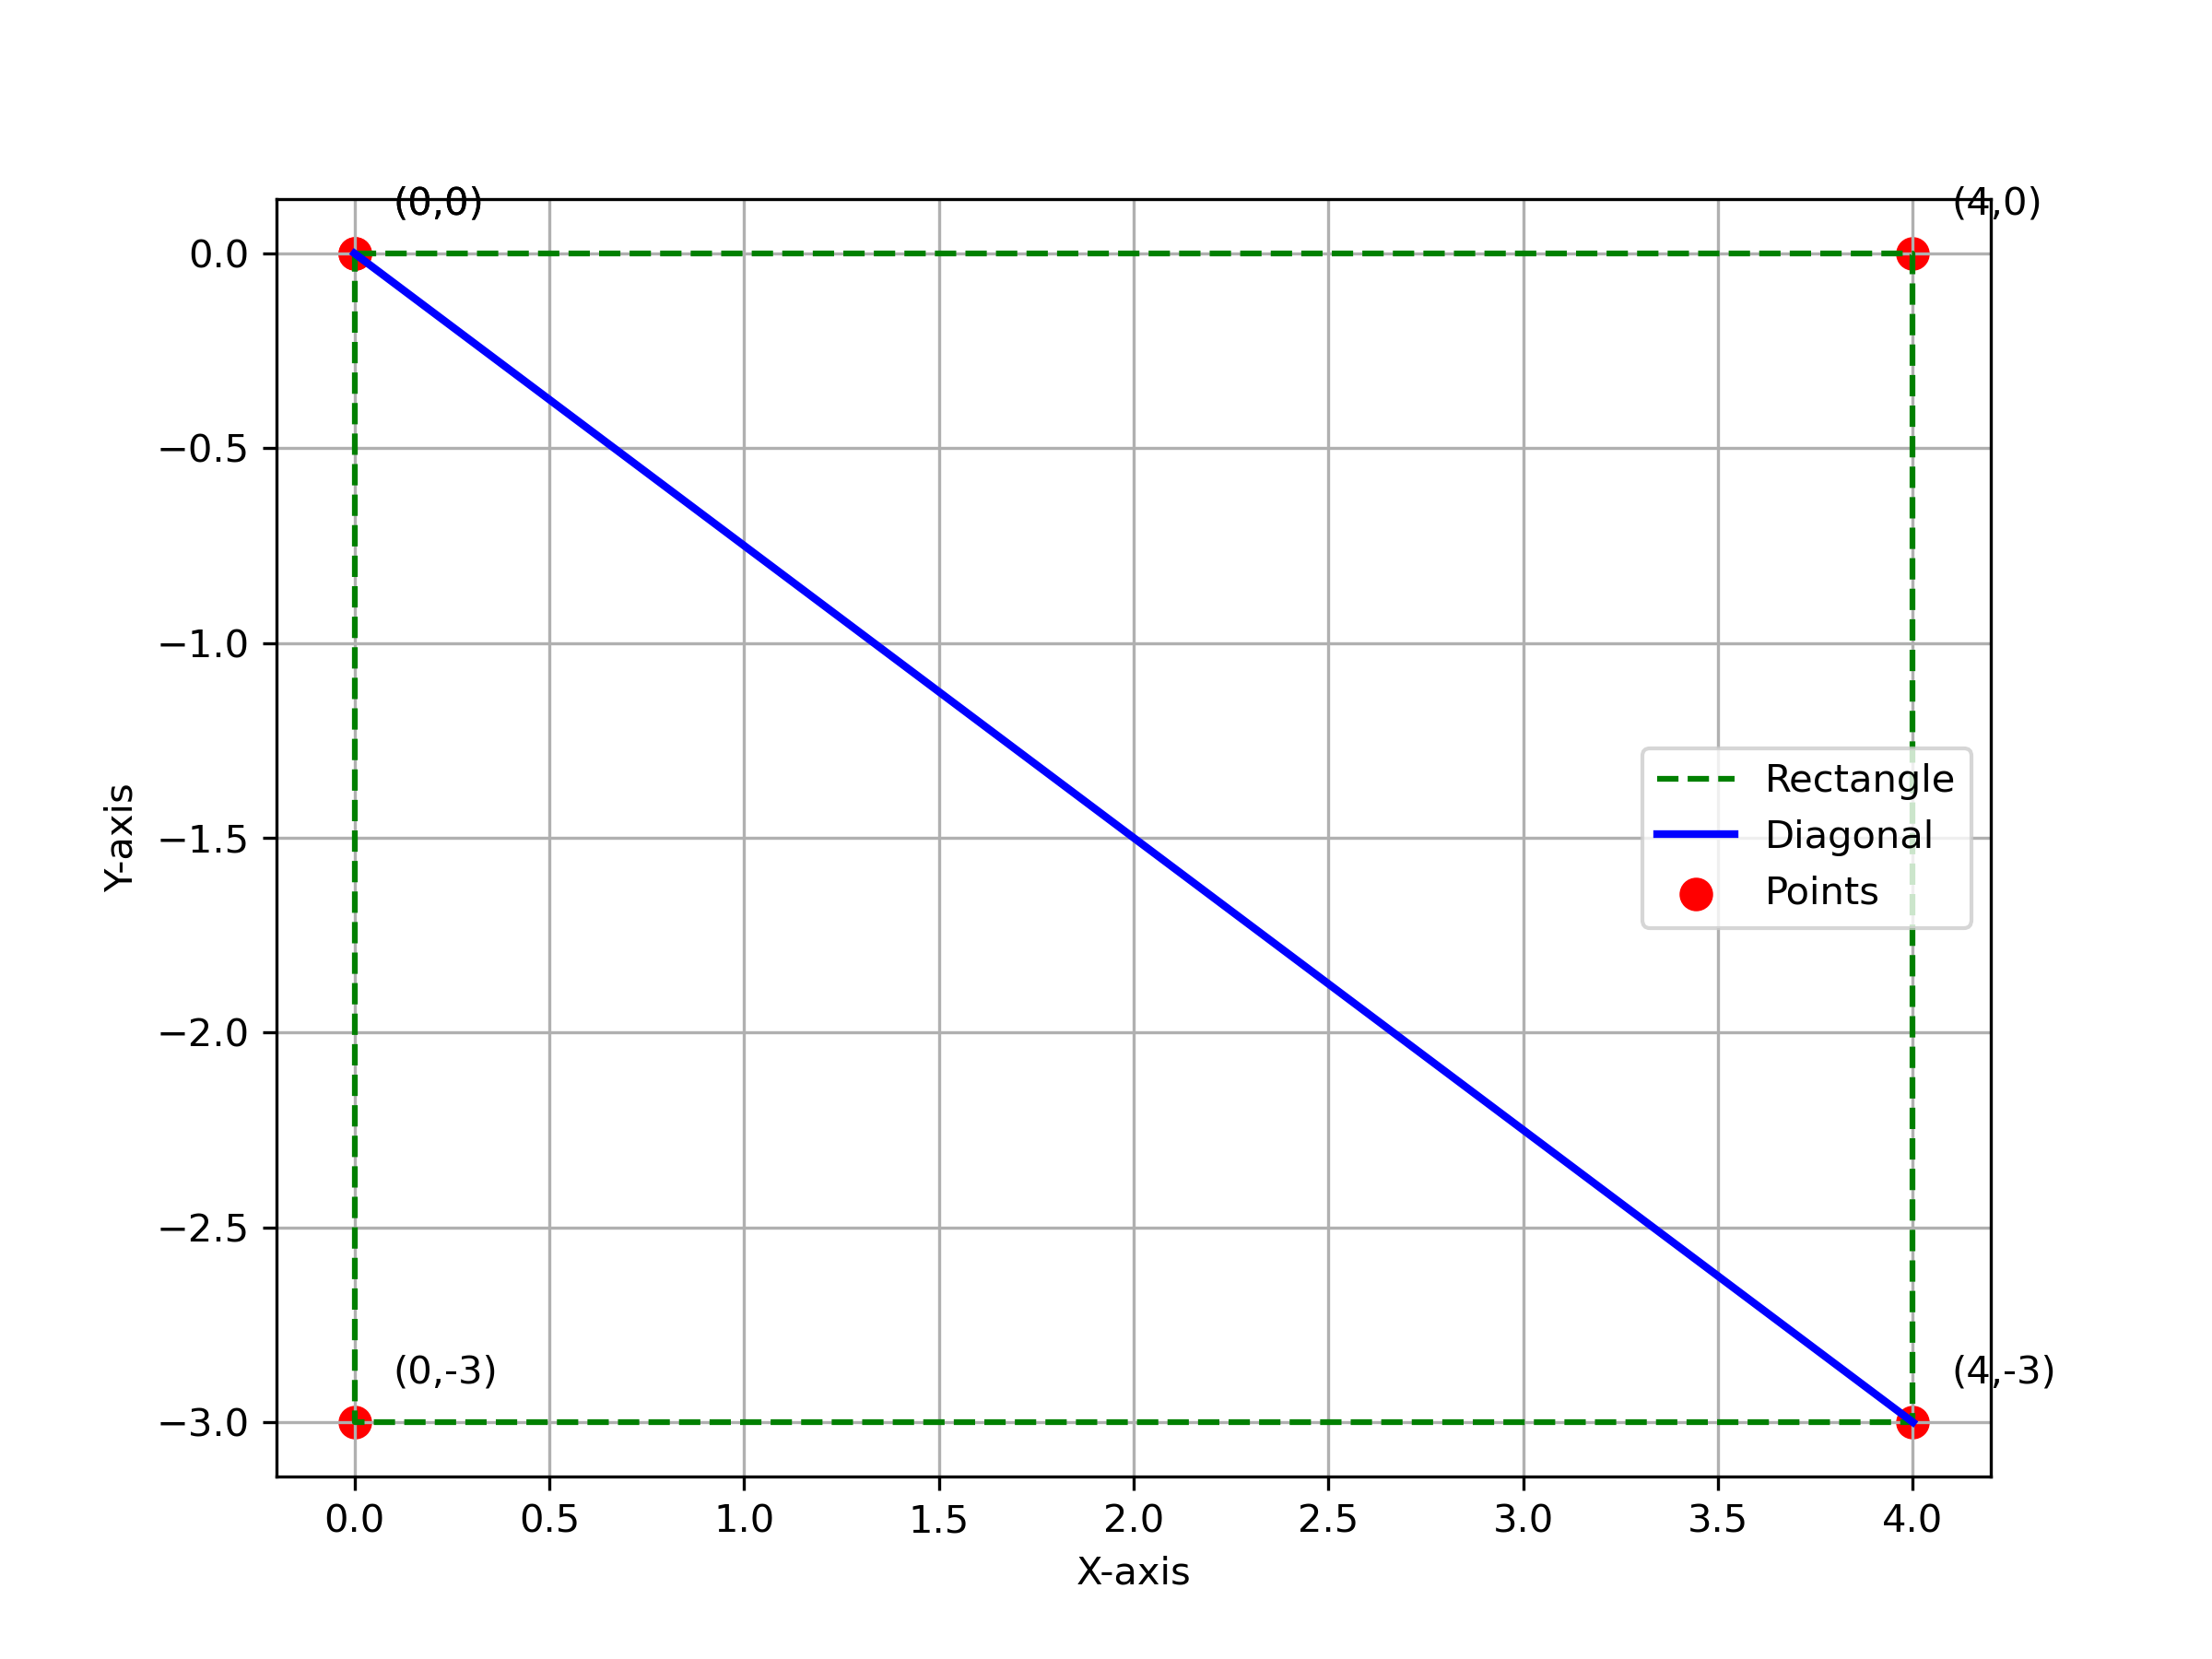
\includegraphics[width=\columnwidth, height=0.8\textheight, keepaspectratio]{../Figs/fig2.png}     
\end{frame}


\end{document}
